\documentclass{article}
\usepackage{graphicx} % Required for inserting images

\usepackage{darkmode}
\usepackage{tikz}

\usepackage{geometry}

\usepackage{amsmath}

\sloppy
% \enabledarkmode

\colorlet{boxfillcolor}{gray!10}

\title{Calc II notes}
\author{Pierson Lipschultz}
\date{March 2025}

\begin{document}



\vspace*{\fill}
\begingroup
\begin{center}
    \huge
    Calc II Notes

    Pierson L
    
\end{center}

\endgroup
\vspace*{\fill}

\pagebreak

\vspace*{\fill}
\begingroup

    \resizebox{\textwidth}{!}{
        \centering
        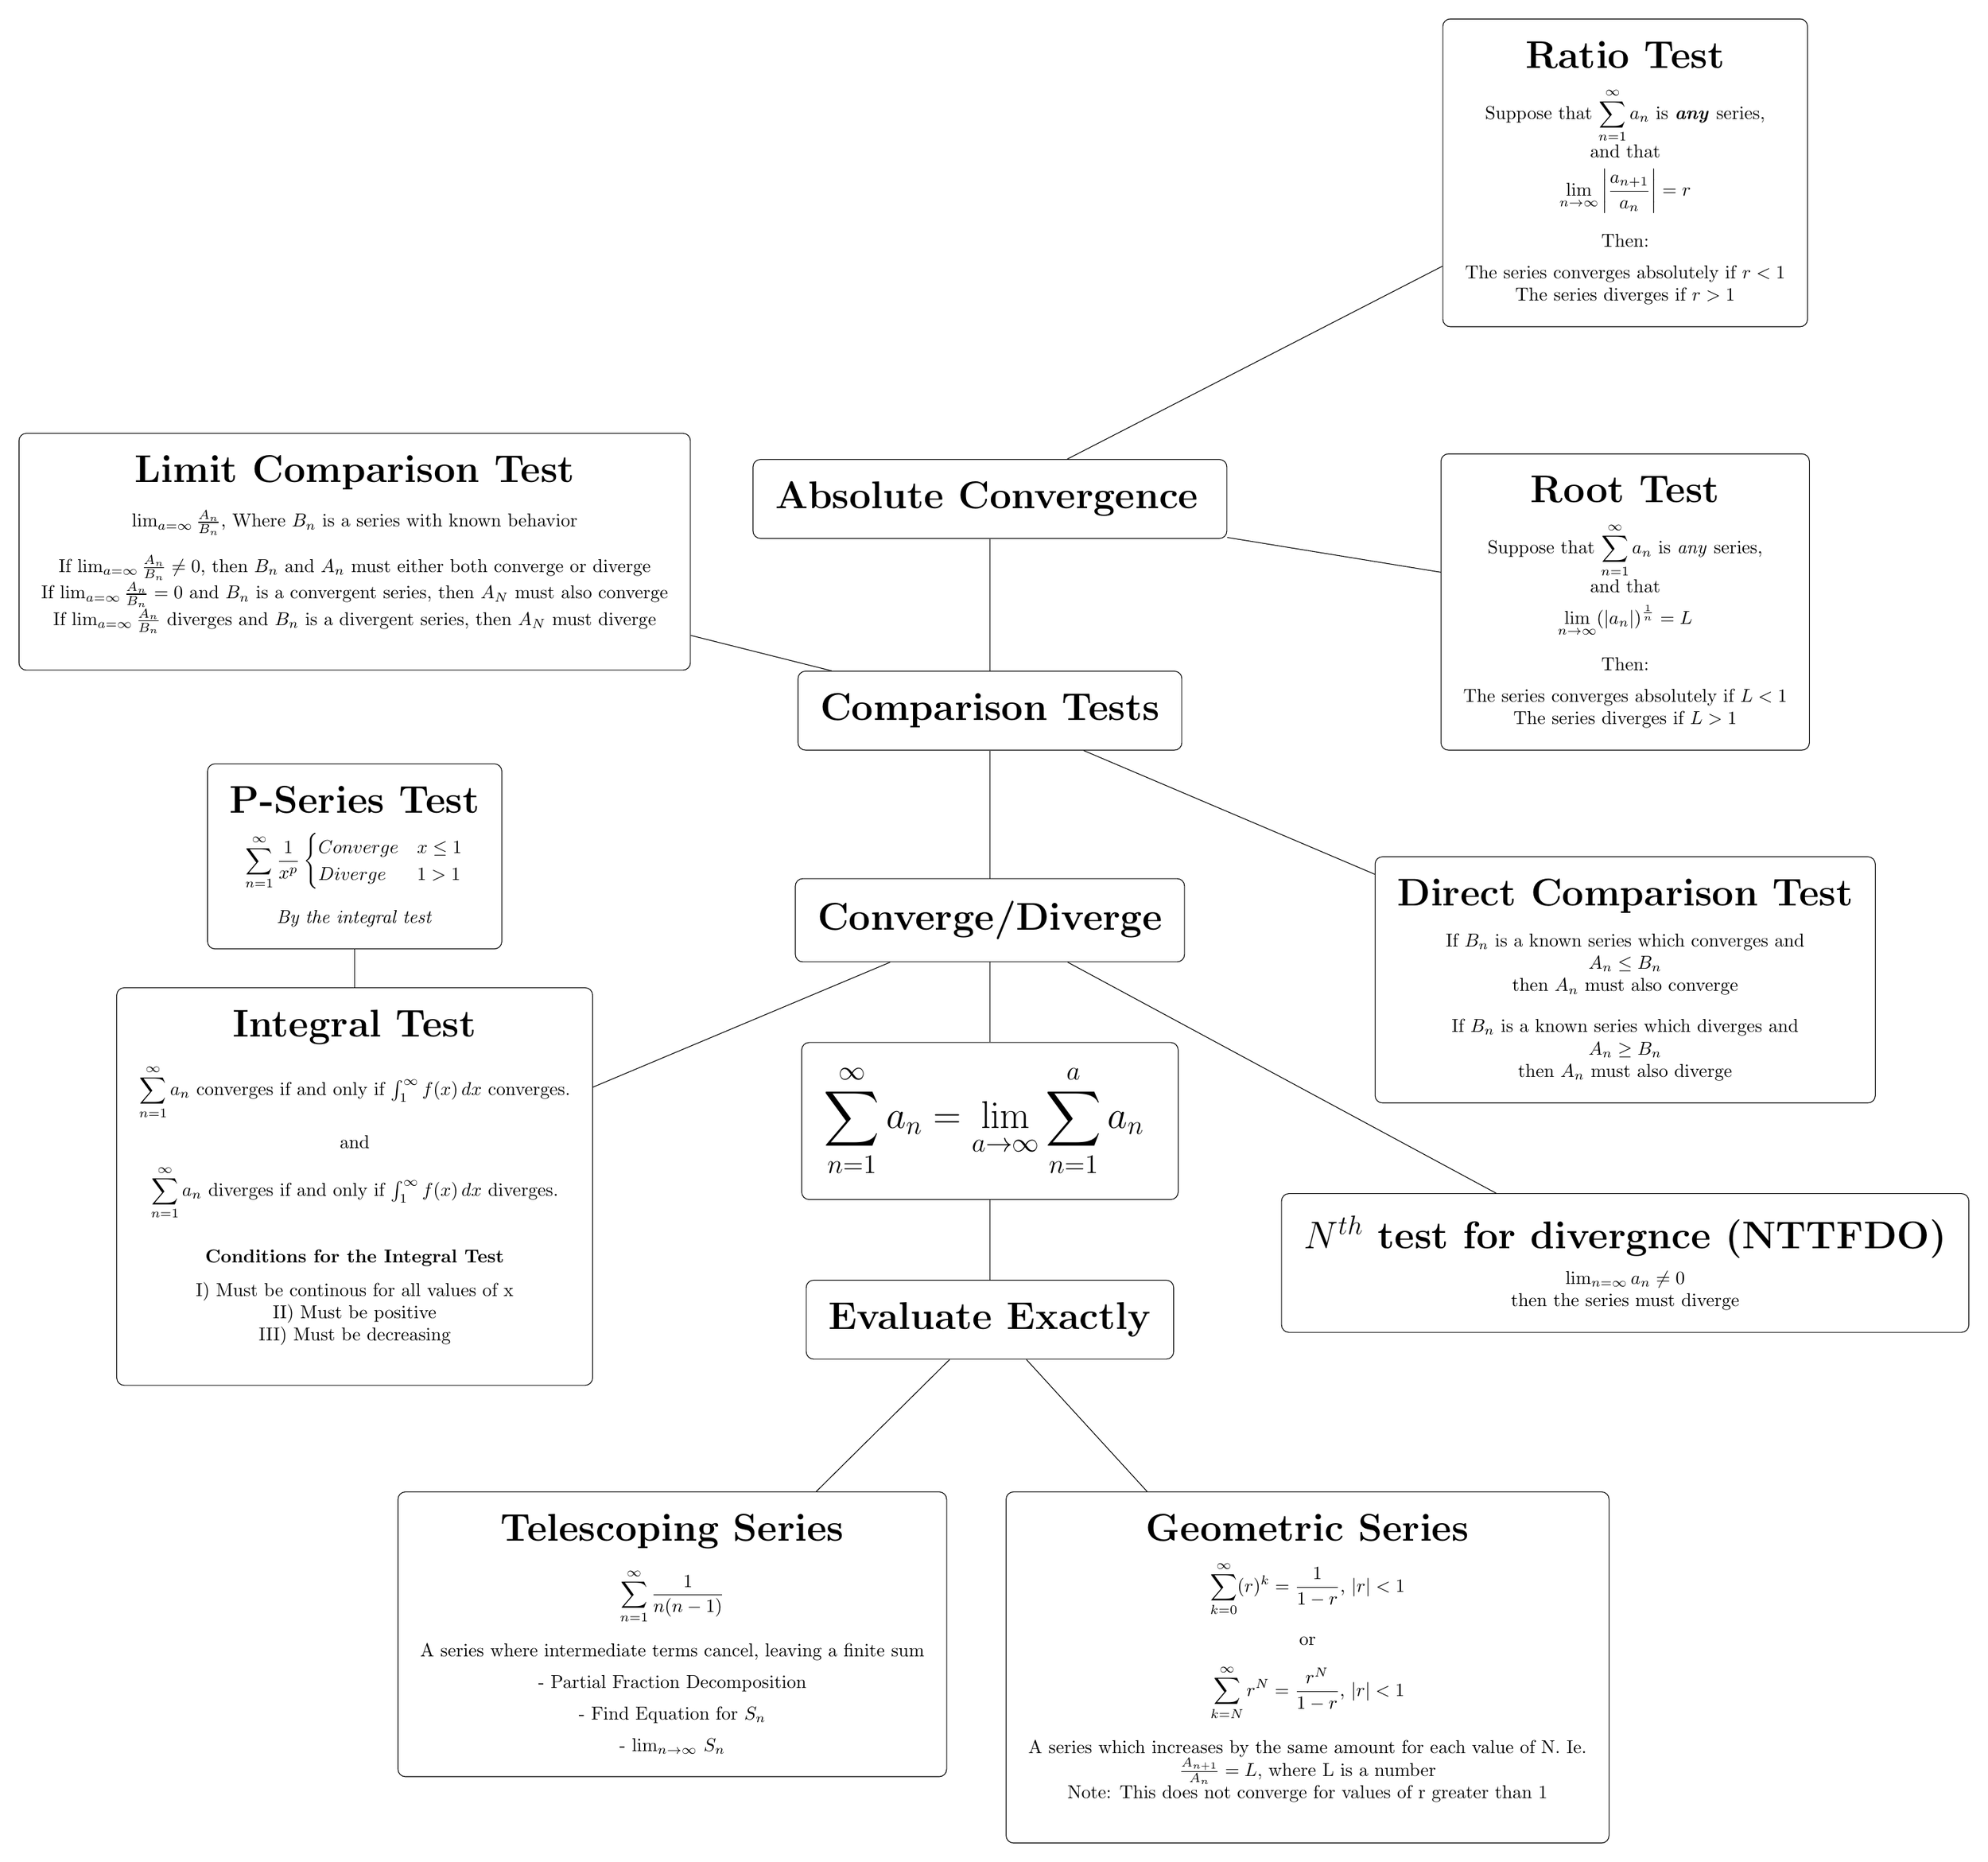
\begin{tikzpicture}

            %titles and jazz

            %main
            \node[shape=rectangle, draw=black, align=center, rounded corners, inner sep=12pt] (Main) at (0,0) {
                \huge $\displaystyle \sum_{n=1}^{\infty} a_n = \lim_{a \rightarrow \infty}\sum_{n=1}^{a} a_n$
            };

            %evalulate 
            \node[shape=rectangle, draw=black, align=center, anchor=north, rounded corners, inner sep=12pt](EvalExc) at (0,-3) {\huge \textbf{Evaluate Exactly}};

            %Converge or Diverge
            \node[shape = rectangle, draw=black, align=center, anchor=south, rounded corners, inner sep=12pt] (CorD) at (0,3){\huge \textbf{Converge/Diverge}};
            
            %NTTFDO
            \node[shape = rectangle, draw=black, align=center, anchor=south, rounded corners, inner sep=12pt] (NTTFDO) at (12,-4){\huge \textbf{$N^{th}$ test for divergnce (NTTFDO)} \\ [6pt] 
            $\lim_{n=\infty} a_n \neq 0$ \\
            then the series must diverge
            };
            
            %Comp tests
            \node[shape = rectangle, draw=black, align=center, anchor=south, rounded corners, inner sep=12pt] (CompT) at (0,7){\huge \textbf{Comparison Tests}};

            %limit comp text
            \node[shape = rectangle, draw=black, align=center, anchor=north, rounded corners, inner sep=12pt] (LCT) at (-12,13){
                {\huge \textbf{Limit Comparison Test}} \\[10pt]
                $\lim_{ a = \infty} \frac{A_n}{B_n}$, Where $B_n$ is a series with known behavior\\ [10pt]
                If $\lim_{ a = \infty} \frac{A_n}{B_n}\neq 0$, then $B_n$ and $A_n$ must either both converge or diverge\\
                If $\lim_{ a = \infty} \frac{A_n}{B_n} = 0$ and $B_n$ is a convergent series, then $A_N$ must also converge\\
                If $\lim_{ a = \infty} \frac{A_n}{B_n}$ diverges and $B_n$ is a divergent series, then $A_N$ must diverge\\

            };

            %direct comp text
            \node[shape = rectangle, draw=black, align=center, anchor=north, rounded corners, inner sep=12pt] (DCT) at (12,5){
                {\huge \textbf{Direct Comparison Test}}\\[10pt]
                If $B_n$ is a known series which converges and\\
                $A_n \leq B_n$\\
                then $A_n$ must also converge\\[10pt]

                If $B_n$ is a known series which diverges and\\
                $A_n \geq B_n$\\
                then $A_n$ must also diverge
            };

            %Absolute convergence 
            \node[shape = rectangle, draw=black, align=center, anchor=south, rounded corners, inner sep=12pt] (ABSConvg) at (0,11){
                {\huge \textbf{Absolute Convergence}}
                };
                
            %Ratio Test
            \node[shape = rectangle, draw=black, align=center, anchor=south, rounded corners, inner sep=12pt] (RatioTest) at (12,15){
                {\huge \textbf{Ratio Test}}\\[10pt]
                Suppose that $\displaystyle \sum_{n=1}^{\infty} a_n$ is \textit{\textbf{any}} series,\\
                and that\\[5pt]
                $\displaystyle \lim_{n \rightarrow \infty} \left| \frac{a_{n+1}}{a_n} \right| = r$\\[10pt]
                Then: \\[5pt]
                The series converges absolutely if $r < 1$\\
                The series diverges if $r > 1$
                };

            %Root Test
            \node[shape = rectangle, draw=black, align=center, anchor=south, rounded corners, inner sep=12pt] (RootTest) at (12,7){
                {\huge \textbf{Root Test}}\\[10pt]
                Suppose that $\displaystyle \sum_{n=1}^{\infty} a_n$ is \textit{any} series,\\
                and that\\[5pt]
                $\displaystyle \lim_{n \rightarrow \infty} ({|a_n|})^\frac{1}{n} = L$\\[10pt]
                Then: \\[5pt]
                The series converges absolutely if $L < 1$\\
                The series diverges if $L > 1$
                };

            %Telescoping
            \node[shape=rectangle, draw=black, align=center, anchor=north, rounded corners, inner sep=12pt] (Tele) at (-6,-7) {
                \textbf{\huge Telescoping Series} \\[10pt]
                $\displaystyle \sum_{n=1}^{\infty} \frac{1}{n(n-1)}$ \\[10pt]
                A series where intermediate terms cancel, leaving a finite sum \\[5pt]
                - Partial Fraction Decomposition  \\[5pt]
                - Find Equation for $S_n$ \\[5pt]
                - $\lim_{n \to \infty}$ $S_n$
            };

            %Geometric
            \node[shape=rectangle, draw=black, align=center, anchor=north, rounded corners, inner sep=12pt] (Geom) at (6,-7) {
                \textbf{\huge Geometric Series} \\[10pt]
                $\displaystyle \sum_{k=0}^{\infty} (r)^k = \frac{1}{1-r},$ $|r| < 1 $ \\[10pt] 
                or \\[10pt]
                $\displaystyle \sum_{k=N}^{\infty} r^N = \frac{r^N}{1-r}, $ $|r| < 1 $\\[10pt]
                A series which increases by the same amount for each value of N. Ie. \\
                $\frac{A_{n+1}}{A_n} = L$, where L is a number \\ 
                Note: This does not converge for values of r greater than 1  \\
            };

            %Integral Test
            \node[shape = rectangle, draw=black, align=center, anchor=south, rounded corners, inner sep=12pt] (IntTest) at (-12,-5){\huge \textbf{Integral Test} \\ [10pt]
            $\displaystyle \sum_{n=1}^{\infty} a_n$ converges if and only if $\int_1^\infty f(x) \, dx$ converges. \\ [8pt]
            and \\ [8pt]
            $\displaystyle \sum_{n=1}^{\infty} a_n$ diverges if and only if $\int_1^\infty f(x) \, dx$ diverges. \\ [15pt]

            \textbf{Conditions for the Integral Test} \\ [6pt]
            I) Must be continous for all values of x\\
            II) Must be positive\\
            III) Must be decreasing \\ 

            };

            %p-series test
            \node[shape = rectangle, draw=black, align=center, rounded corners, inner sep=12pt] (PSes) at (-12,5){\huge \textbf{P-Series Test}\\ [10pt]
            
            $\displaystyle \sum_{n=1}^{\infty} \frac{1}{x^p} \begin{cases} 
            Converge & x\leq 1 \\
            Diverge & 1 > 1 \\ 
            \end{cases}$ \\ [10pt]
            
            \textit{By the integral test} 
            };




            \path [-] (Main) edge node[left] {$$} (EvalExc);
            \path [-] (EvalExc) edge node[left] {$$} (Tele);
            \path [-] (EvalExc) edge node[left] {$$} (Geom);
            \path [-] (Main) edge node[left] {$$} (CorD);
            \path [-] (CorD) edge node[left] {$$} (NTTFDO);
            \path [-] (CorD) edge node[left] {$$} (IntTest);
                \path [-] (IntTest) edge node[left] {$$} (PSes);
            \path [-] (CorD) edge node[left] {$$} (CompT);
                \path [-] (CompT) edge node[left] {$$} (LCT);
                \path [-] (CompT) edge node[left] {$$} (DCT);
                \path [-] (CompT) edge node[left] {$$} (ABSConvg);
                    \path [-] (ABSConvg) edge node[left] {$$} (RatioTest); 
                    \path [-] (ABSConvg) edge node[left] {$$} (RootTest); 



        \end{tikzpicture}
    }

\endgroup
\vspace*{\fill}

\pagebreak
\title{Absolute Convergence}
    \section{Ratio Test} 
    \hrulefill \\[10pt]

    The Ratio Test\footnote{Very important regarding factorials} states that 
        
        \begingroup
        \centering
        Suppose that $\displaystyle \sum_{n=1}^{\infty} a_n$ is \textit{\textbf{any}} series,\\
        and that\\[5pt]
        $\displaystyle \lim_{n \rightarrow \infty} \left| \frac{a_{n+1}}{a_n} \right| = r$\\[10pt]
        Then: \\[5pt]
        The series converges absolutely if $r < 1$\\
        The series diverges if $r > 1$\\
        \endgroup

    \subsection{Examples}

        \begingroup
        \centering

        \fbox{\large \textbf{ex. 1}}\\

        \hrulefill \\[10pt]

        \fbox{\large Simplify $\frac{(n+2)!}{(n-1)!}$}\\[5pt]
        \textit{Ratio of factorials}\\[15pt]

        $=\frac{(n+2)!}{(n-1)!}$\\[15pt]
        
        $= \frac{(n+1)(n+1)(n)(n-1)\cdots(1)}{(n-1)(n-2)(n-3)\cdots(1)}$\\[15pt]
        
        $= \frac{(n+1)(n+1)(n)(n-1)}{(n-1)}$\\[15pt]

        $= {(n+1)(n+1)(n)}$\\[15pt]

        \endgroup
    \pagebreak



\title{Misc}
    \centering
    \subsection{\huge Factorials}
    \fbox{\large ex.1}

        \hrulefill \\[10pt]

            \fbox{\large 4! = 4 x 3! = 4x3x2! = 4x3x2x1! = 4x3x2x1x0!}

            $\rightarrow$

            \fbox{0! = 1}

            $\rightarrow$

            \fbox{4!= 24}

            \hrulefill \\[10pt]

    \fbox{\large \textbf{ex. 2}}\\

    \hrulefill \\[10pt]

    \fbox{\large Simplify $\frac{(n+2)!}{(n-1)!}$}\\[5pt]
    \textit{Ratio of factorials}\\[15pt]

    $=\frac{(n+2)!}{(n-1)!}$\\[15pt]
    
    $= \frac{(n+1)(n+1)(n)(n-1)\cdots(1)}{(n-1)(n-2)(n-3)\cdots(1)}$\\[15pt]
    
    $= \frac{(n+1)(n+1)(n)(n-1)}{(n-1)}$\\[15pt]

    $= {(n+1)(n+1)(n)}$\\[15pt]
\end{document}
